\section{System Evaluation and Analysis}

\subsection{Test Case}
In this section, we will show how to use our website by showing the process of how a patient goes to see doctor in hospital, as an evaluation of the whole system. All roles except administrator will be involved in this process. Considering that we have already discussed administrator’s functionality in Section \ref{sec:admin}. We won’t talk about it again.
\begin{figure}[H]
    \centering
    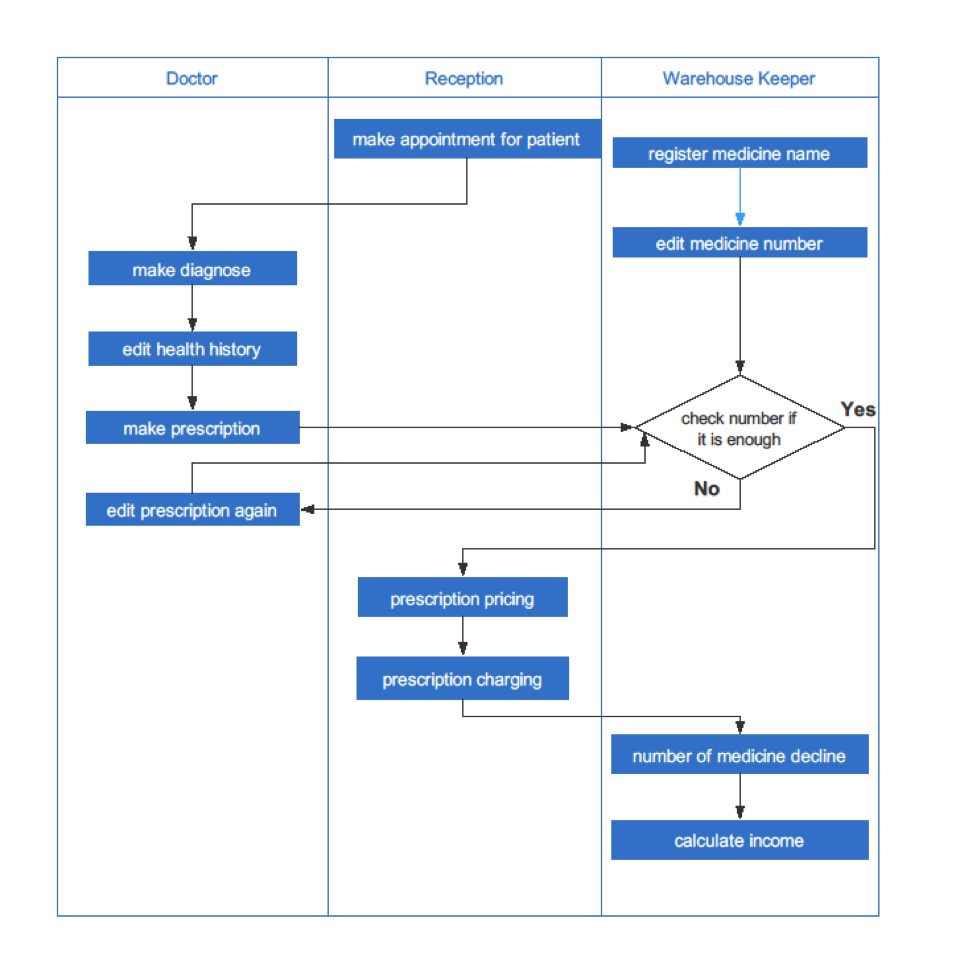
\includegraphics[width=\textwidth]{pp/pp1.jpg}
    \caption{Process}
    \label{fig:pp1}
\end{figure}
\begin{enumerate}
    \item When a patient enters the hospital, he first talks to a reception at front desk. And the reception will visit \emph{patient making appointment} page and create a health history record.
    \begin{figure}[H]
    \centering
    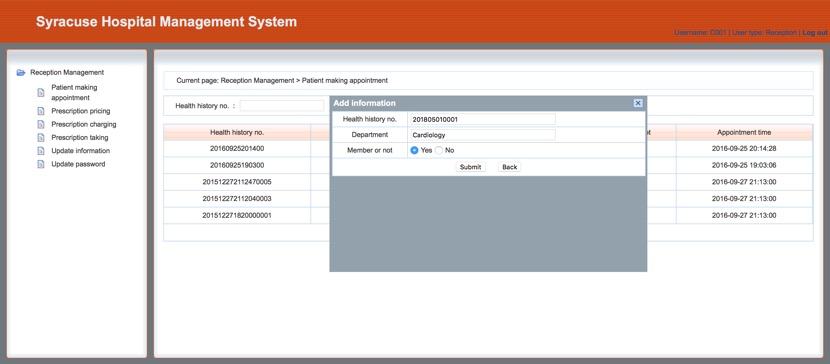
\includegraphics[width=\textwidth]{pp/pp2.jpg}
    \caption{patient making appointment}
    \label{fig:pp2}
\end{figure}
    \item Then the patient will visit the doctor. After the record is created, it will automatically appear in doctor’s \emph{Edit health history} Page, and doctor can edit it.
    \begin{figure}[H]
    \centering
    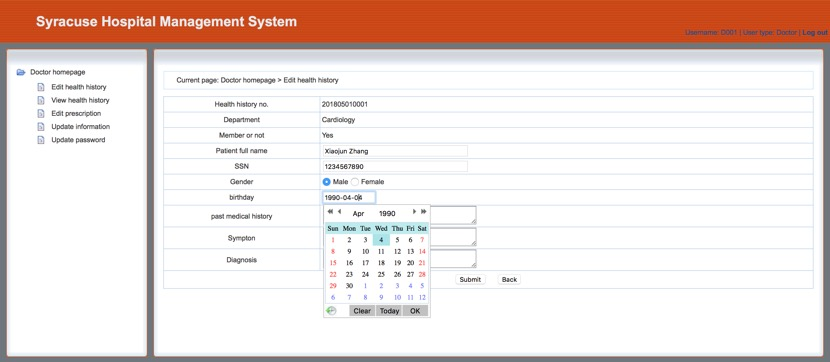
\includegraphics[width=\textwidth]{pp/pp3.jpg}
    \caption{Edit health history}
    \label{fig:pp3}
\end{figure}
    \item After editing the history, doctor can still review it in \emph{View health history} page.
    \begin{figure}[H]
    \centering
    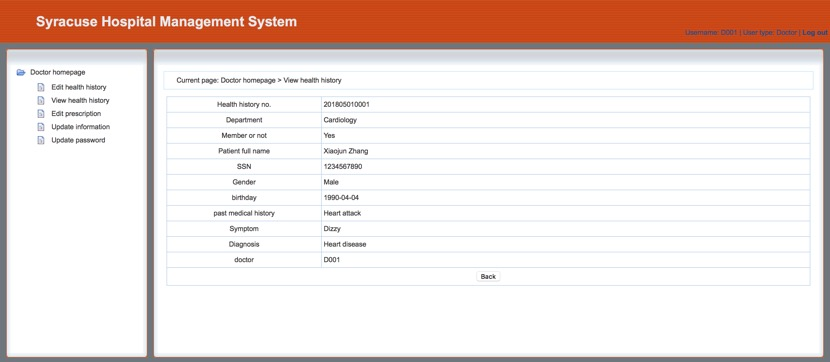
\includegraphics[width=\textwidth]{pp/pp4.jpg}
    \caption{View health history}
    \label{fig:pp4}
\end{figure}
    \item Then doctor will create a prescription for this health history. Mentioning that if doctor want to use multiple different kinds of medicines, he just have to add multiple times with certain quantities.
    \begin{figure}[H]
    \centering
    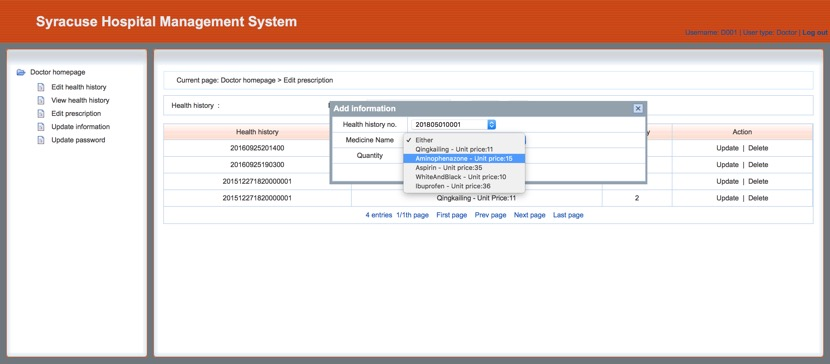
\includegraphics[width=\textwidth]{pp/pp5.jpg}
    \caption{Edit prescription}
    \label{fig:pp5}
\end{figure}
    \item Now the patient can go back to see the reception again. The reception will visit \emph{Prescription pricing}, \emph{Prescription charging} and \emph{Prescription taking} page one by one to help the patient to pay for and to fetch medicine. 
    \begin{figure}[H]
    \centering
    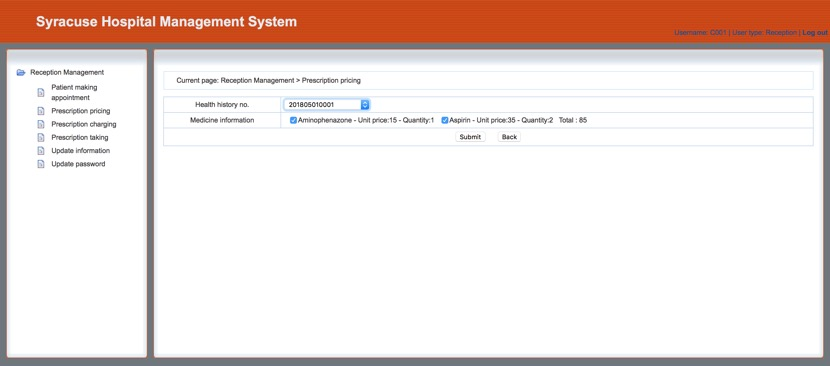
\includegraphics[width=\textwidth]{pp/pp6.jpg}
    \caption{Prescription pricing}
    \label{fig:pp6}
\end{figure}
    \begin{figure}[H]
    \centering
    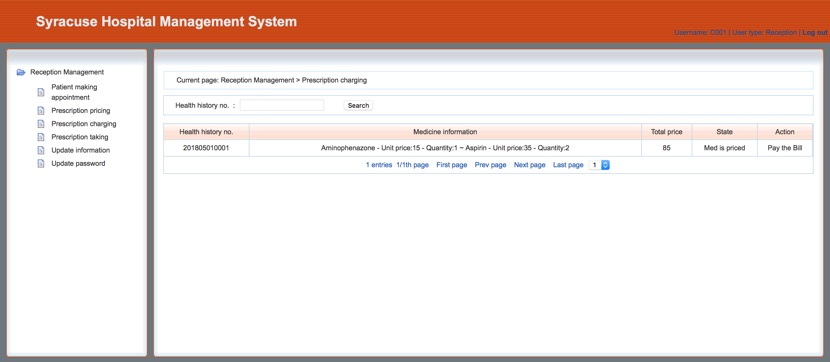
\includegraphics[width=\textwidth]{pp/pp7.jpg}
    \caption{Prescription charging}
    \label{fig:pp7}
\end{figure}    \begin{figure}[H]
    \centering
    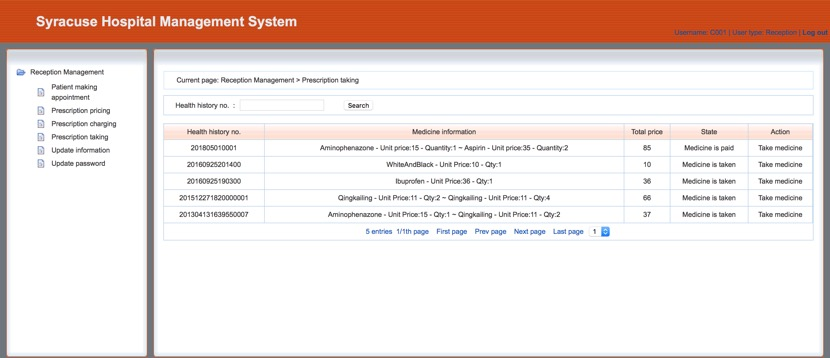
\includegraphics[width=\textwidth]{pp/pp8.jpg}
    \caption{Prescription taking}
    \label{fig:pp8}
\end{figure}
    \item We can check \emph{Medicine summary} page before and after process 1 to 5. And we will see that the \emph{current inventory} row is decreased after this process.
\begin{figure}[H]
    \centering
    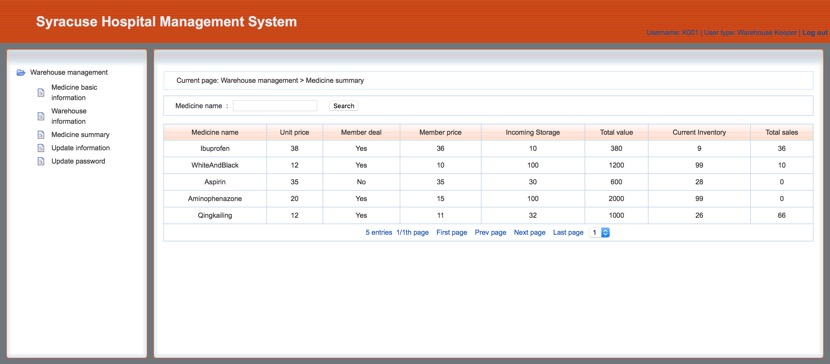
\includegraphics[width=\textwidth]{pp/pp9.jpg}
    \caption{Medical Summary}
    \label{fig:pp9}
\end{figure}
\end{enumerate}

\subsection{Main functionality}
\subsubsection{Main functionality}

This project focus on the information processing problems in real-time hospital scenarios, including the whole process from appointment to prescription. And our main goal is to achieve rapid response and high efficiency in hospital information management situations. The system mainly includes user management, medical record management, prescription management, warehouse management, log management, etc.

\subsubsection{Details}
\begin{itemize}
    \item Based on the actual demand in hospital situation, we conclude the lightweight design of the hospital management system, which achieves low system requirements.
    \item we choose moderate open-source MySQL as our database management system and connect it with basic JDBC API, which provide with easy adoption and scalability support based on further demands.
    \item Roles defined in the system are clearly separated and the functionality of  modules can meet the requirements of hospital scenarios. Our UI design is concise, clear and user-friendly, thus users can easily find the information and finish their operations without additional guidance.
    \item Thanks to the strong capability and cross-platform functionality of Java, our system can be implemented on various platforms, and support multiple devices with little effort.
    \item We implement several security countermeasures to eliminate the risk of various potential attacks, including SQL injection attack, CSRF and XSS attack. Therefore our system provide sufficient protection on sensitive information and user credentials in terms of confidentiality and integrity.
\end{itemize}

\subsection{Features}
\subsubsection{Log Management}
Event logs record events taking place in the execution of a system in order to provide an audit trail that can be used to understand the activity of the system, to diagnose problems and to recover from incorrect actions. In our hospital management system, we keep record of all employee actions, such as login, creating prescription and medicine into warehouse.

With this log table, the website is much more maintainable for administrator
\begin{figure}[H]
    \centering
    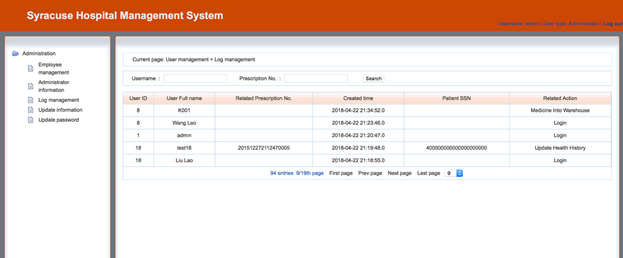
\includegraphics[width=\textwidth]{fp/s1.png}
    \caption{Log Management}
    \label{fig:sp1}
\end{figure}
\subsubsection{Coherence and streamlined}
It is our goal to design a highly efficient and practical health center management website, which means that different roles don’t have to consider interaction with other roles and that our server will assist them to achieve interaction. Therefore, coherence is an import part of our design. There is coherence everywhere in our system.
\begin{figure}[H]
    \centering
    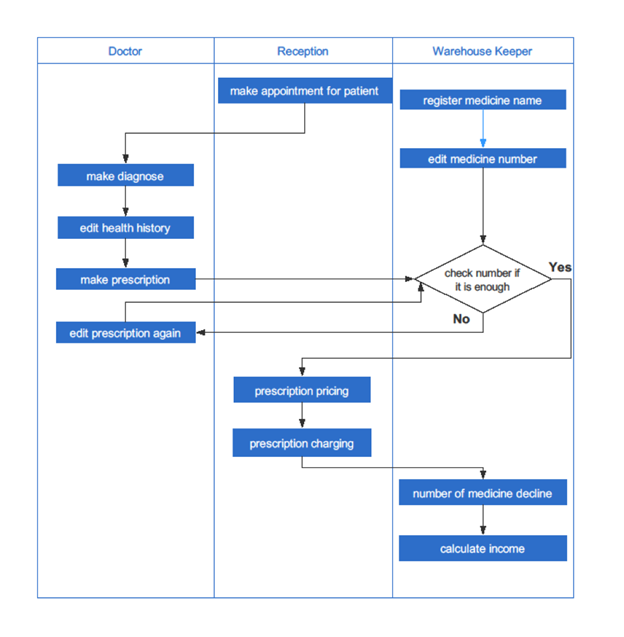
\includegraphics[width=\textwidth]{fp/s2.png}
    \caption{Coherence}
    \label{fig:sp2}
\end{figure}
\begin{enumerate}
    \item Reception and Doctor
    
    After a reception makes an appointment for a patient, a fresh unedited health  history record will automatically be created in doctors’s \emph{edit health history page}. After editing it, a doctor can create prescription for this history record. After that, a prescription will automatically appear in reception’s \emph{prescription pricing} page. 
    \begin{figure}[H]
    \centering
    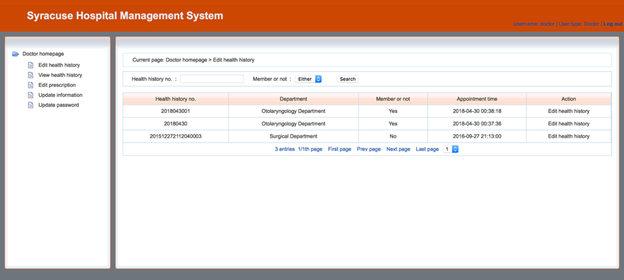
\includegraphics[width=\textwidth]{fp/s3.png}
    \caption{Edit health history record}
    \label{fig:sp3}
\end{figure}
    \item Reception and Warehouse Keeper
    
    After a reception charges and takes medicine for a patient. This action is automatically record to our database, and the amount of available medicine in the warehouse is automatically decreased.
\end{enumerate}

\subsubsection{Detail oriented}
To make our website as real and practical as possible, we focus on detail as best as we can. 

\begin{itemize}
    \item We make updating password logic and all other actions atomic and rigorous. 
    \item We apply a lot of format constraints to simulate real personal information.
        \begin{figure}[H]
    \centering
    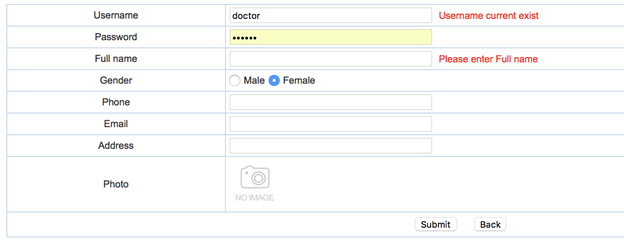
\includegraphics[width=\textwidth]{fp/s5.png}
    \caption{Constraint 1}
    \label{fig:sp5}
\end{figure}
\begin{figure}[H]
    \centering
    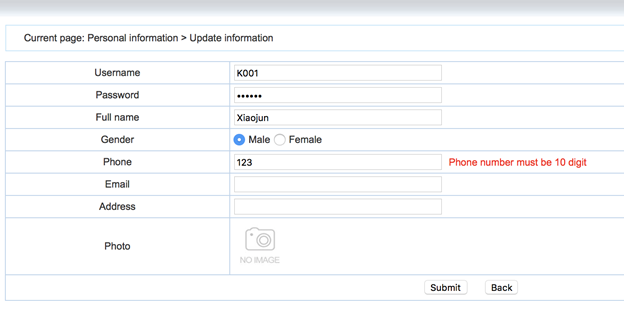
\includegraphics[width=\textwidth]{fp/s6.png}
    \caption{Constraint 2}
    \label{fig:sp6}
\end{figure}
\begin{figure}[H]
    \centering
    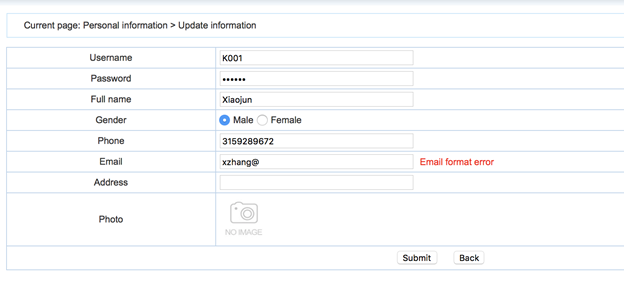
\includegraphics[width=\textwidth]{fp/s7.png}
    \caption{Constraint 3}
    \label{fig:sp7}
\end{figure}
\end{itemize}

